\medskip

\textbf{Partie A : }

\begin{enumerate}
\item D'une part :  $\begin{cases}
\lim\limits_{x \to -1^+} x+1 = 0^+ \\
\lim\limits_{X \to 0} \ln X = -\infty
\end{cases}$ donc par composition $\lim\limits_{x \to -1} 4\ln (x+1) =-\infty$ 

D'autre part, $\lim\limits_{x \to -1}\dfrac{-x^2}{25}= -\dfrac{1}{25}$ 

donc par somme $\lim\limits_{x \to -1}f(x) = -\infty$



\item $f$ est dérivable sur $]-1~;~+\infty[$.

$f$ est de la forme $4\ln(u) - v$ avec $u(x) = x + 1$ et $v(x) = \dfrac {x^2}{25}$.

On a  $u'(x) =1$ et $v'(x)= \dfrac{2x}{25}$

Or $f'= 4 \dfrac{u'}{u}-v'$ donc :

Pour tout $x$ appartenant à l'intervalle $]-1 ;+\infty[$, on a :

$f'(x) = 4 \dfrac{1}{x+1}- \dfrac{2x}{25}= \dfrac{4 \times 25 -(x+1)2x}{25(x+1)}= \dfrac{100-2 x-2 x^{2}}{25(x+1)}
$
\item Pour tout $x$ appartenant à l'intervalle $]-1 ;+\infty[$, on a :

$f'(x) = \dfrac{100-2 x-2 x^{2}}{25(x+1)}$ 

$25(x+1)>0$ donc $f'(x)$ est du signe de $100 - 2x - 2x^2$, fonction polynôme du second degré donc le coefficient dominant ($-2$) est négatif.

$\Delta = (-2)^2-4 \times 100 \times (-2)= 804 > 0$

$100-2x-2x^2=0$ admet donc deux racines :

$x_1 = \dfrac{2-\sqrt{804}}{2(-2)}= \dfrac{-1+\sqrt{201}}{2} \approx 6,6$

et $x_2 = \dfrac{2+\sqrt{804}}{2(-2)}= \dfrac{-1-\sqrt{201}}{2} \approx -7,6 <-1$

On obtient donc le tableau de variations suivant :

\hfill~	\begin{tikzpicture}
\tkzTab[lgt=3,deltacl=0.6]{$x$ / 0.7 , signe de $f'(x)$ / 0.7, variations de $f$ / 1.5}{$-1$, $x_1$, $+\infty$}
{d, +, z, -, }
{D- / $-\infty$, +/ $f(x_1)$, -/}
\end{tikzpicture}~\hfill~

$[2~;~6,5] \subset ]-1~;~x_1[$ donc $f$ est strictement croissante sur $[2~;~6,5]$.

\item $h(2) =f(2) - 2 = 4 \ln (2+1)-\dfrac{2^{2}}{25}-2 \approx 2,23$.

Sur l'intervalle $[2~;~m]$ la fonction $h$ est strictement croissante, or $h(2)>0$ donc sur $[2~;~m]$, $h(x)>0$ et l'équation $h(x)=0$ n'admet pas de solution sur cet intervalle.

Sur l'intervalle $[m~;~6,5]$, la fonction $h$ est strictement décroissante et continue.

$h(m) = M \approx 2,265 > 0$

et $h(6,5)=4 \ln (6,5+1)-\dfrac{6,5^{2}}{25} -6,5 \approx -0,13 <0$

0 est donc une valeur intermédiaire entre $h(m)$ et $h(6,5)$, 
d'après le théorème des valeurs intermédiaires appliqué aux fonctions strictement monotone, l'équation $h(x)=0$ admet une unique solution $\alpha$  sur l'intervalle $[m~;~6,5]$.

Finalement, l'équation $h(x)=0$ admet une unique solution $\alpha$ sur l'intervalle $[2~;~6,5]$.
\item
	\begin{enumerate}
		\item Avec la calculatrice, on trouve que les valeurs renvoyées par la commande bornes (2) sont : (6.36, 6.37)
		\item Dans le contexte de l'exercice, un encadrement de $\alpha$ est $6,36 < \alpha < 6,37$.
	\end{enumerate}
\end{enumerate}

\medskip

\textbf{Partie B :}

\medskip

\begin{enumerate}
\item Pour tout entier naturel  $n$, on pose $P_n$, l'affirmation : \og $2 \leqslant u_{n} \leqslant u_{n+1} \leqslant 6,5$. \fg{}.

\textbf{Initialisation :} On a, d'une part : $u_0 =2 $,

Et, d'autre part : $u_1=f(u_0)=f(2)\approx 4,23$

Donc $2 \leqslant u_0 \leqslant u_1 \leqslant 6,5$

Pour $n = 0$, l'affirmation $P_0$ est vraie.

\textbf{Hérédité :} Soit $n$ naturel , tel que  l'affirmation $P_n$  est vraie, c'est-à-dire : \quad \og $2 \leqslant u_{n} \leqslant u_{n+1} \leqslant 6,5$ \fg{}.

On veut montrer que cela implique que l'affirmation $ P_{n+1} $ est vraie.

Par hypothèse de récurrence $2 \leqslant u_{n} \leqslant u_{n+1} \leqslant 6,5$ 

Or la fonction $f$ est strictement croissante sur l'intervalle $[2~;~6,5]$ donc :

$f(2) \leqslant f\left( u_{n} \right) \leqslant f\left( u_{n+1} \right) \leqslant f(6,5)$ 

or $f(2) \approx 4,23 >2$ et $f(6,5) \approx 6,37 < 6,5$

donc, par définition de la suite $u$, $  2 \leqslant u_{n+1} \leqslant u_{n+2} \leqslant 6,5$

c'est l'inégalité  $P_{n+1}$

\textbf{Conclusion :} L'affirmation est vraie au rang 0, et, pour tout rang naturel non nul, sa véracité est héréditaire, donc, en vertu du principe de démonstration par récurrence, on peut vérifier l'inégalité $ P_n $ pour tout entier naturel $n$.
\item Pour tout entier $n$ , $u_n \leqslant u_{n+1}$ donc la suite $(u_n)$ est croissante, 

de plus, pour tout entier $n$, $u_n \leqslant 6,5$ donc la suite $(u_n)$ est majorée, 

or, tout suite croissante et majorée est convergente

donc la suite $\left(u_{n}\right)$ est converge vers une limite $\ell$ telle que $2 \leqslant \ell \leqslant 6,5$.
\item La suite $(u_n)$ est une suite convergente vers une limite $\ell$ de la forme $u_{n+1}=f\left(u_{n}\right)$ avec $f$ fonction continue. 
D'après le théorème du point fixe, la limite $\ell$ est solution de l'équation $f(x)=x$ ou $h(x)=0$ 

On sait de plus que cette limite appartient à l'intervalle $[2;6,5]$ et que sur cette intervalle l'équation $h(x)=0$ admet une unique solution $\alpha$ on a donc $\ell =\alpha$.

\end{enumerate}

\medskip
